\documentclass[pdf,color]{UoBnote}

\author{Andreas Freise}

\shorttitle{Short title}
\title{Title}
\date{\today}
\issue{1}

\begin{document}

\maketitle
\tableofcontents
\vspace{1cm}\hrule \vspace{1cm}
%\newpage

\section{Introduction}

This is just a very simple latex document which shows some of what can be done.
\begin{itemize}
\item Environments
\item Examples
\end{itemize}
\subsection{Mathematic Environments}
\label{se:environments}
You can typset equations in many different ways,
\[
\mathbf{F} = m\mathbf{a}.
\]
Or you can write equations in a line of text $\mathbf{F} = m\mathbf{a}$. \\
If you wanted to include an equation number \dots
\begin{equation}
\mathbf{F} = m\mathbf{a}
\end{equation}
You can even work with multiple lines
\begin{eqnarray}
\mathbf{F} &=& m\mathbf{a} \nonumber \\
&=& m\mathbf{\dot{v}}
\label{eq:newton}
\end{eqnarray}
Reading the .tex file along with this .pdf should point out that there are different environments in which you can type equations such as using eqnarray for equation (\ref{eq:newton}) from section \ref{se:environments}. This is not an extensive list there are many more which can be found on the internet you should hunt out and use `align'.
\subsection{Examples}
Here are a few examples covering basic mathematics you may encounter.

\begin{equation}
f(x,t)=g(x-vt)+h(x+vt)
\end{equation}

\begin{equation}
\mathbf{\nabla}\cdot\mathbf{A}(\mathbf{x},\mathbf{y},\mathbf{z}) = \frac{\partial}{\partial x}\mathbf{A}(\mathbf{r})\hat{x} + \frac{\partial}{\partial y}\mathbf{A}(\mathbf{r})\hat{y} + \frac{\partial}{\partial z}\mathbf{A}(\mathbf{r})\hat{z}
\end{equation}
\begin{eqnarray*}
\ln e^{x} &=& x \\
e^{x} &=& \sum_{n=0}^{\infty}\frac{(x)^{n}}{n!} \\
\ln(x+1) &\approx& x - \frac{x^{2}}{2} + \frac{x^{3}}{3} \hspace{1cm} |x| < 1
\end{eqnarray*}

\section{Another section}

Another  section with a figure and a table.
The figure~\ref{fig:figure1} is \textbf{floating}! Do not try to
control its position yourself!
The table is a simple example, also tables can be floating, however,
the following one is not:
\begin{center}
\begin{tabular}{|l|c|c|}
        \hline
        mode  & LG00 & LG33\\
        \hline
        ratio & 2.63 & 4.31\\
        \hline
\end{tabular}
\end{center}

You can include source code or text output from your programs in the
following way (this example just shows the output of the `ls' command
on a Linux system):
\begin{verbatim}
black:LatexExample adf$ ls
UoBnote.cls        UoBnoteexample.pdf UoBnoteexample.tex beams.pdf          bhamlogo.pdf
black:LatexExample adf$ 
\end{verbatim}


\begin{figure}
\begin{center}
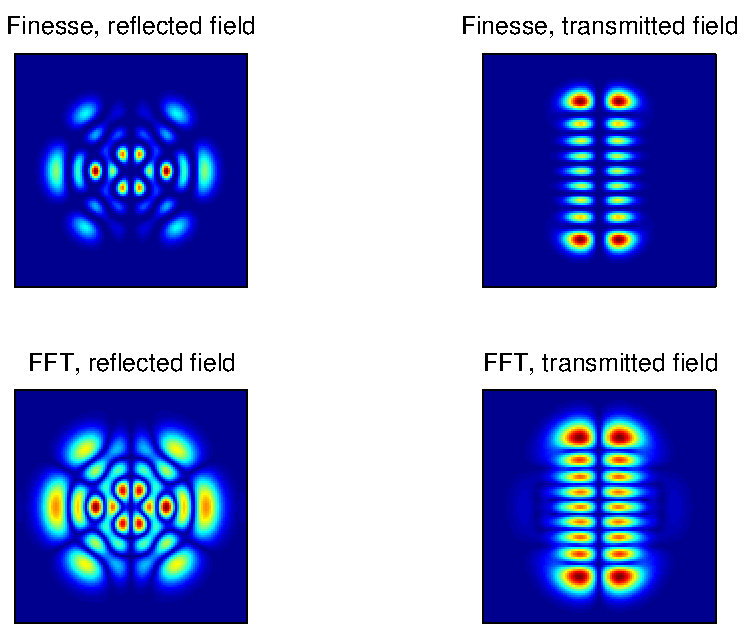
\includegraphics[scale=0.75]{beams.pdf}
\end{center}
\caption{This is an example for including a figure.}\label{fig:figure1}
\end{figure}


\end{document}
